% ------------------------------------------------------------------------------------------- %
%                                         Metodologia                                         %
% ------------------------------------------------------------------------------------------- %
\chapter{Materiais e Métodos}\label{cap:materialemetodos}

\section{Materiais}\label{sec:materiais}

\subsection{CV Lattes}\label{subsec:lattes}

A plataforma Lattes, concebida em agosto de 1999, representa a experiência do \gls{cnpq} na integração de bases de dados de currículos e de instituições da área de ciência e tecnologia em um único sistema de informações, padronizando em ambito nacional o formato para coleta de informações curriculares e cuja importância atual se estende, não só às atividades do \gls{cnpq}, como também às ações de incentivo a outras instituições federais e estaduais \cite{Lattes}.

A plataforma também possui uma página web para busca textual dos currículos cadastrados em seu sistema bem como uma ferramenta para extração de dados de sua base denominado \textit{Lattes Extrator}, porém tal ferramenta só é disponibilizada às instituições que devem efetuar cadastro e solicitar acesso a mesma.

\subsection{PostgreSQL}\label{subsec:postgresql}

O PostgreSQL é um banco de dados relacional contributivo, ou seja, tem seu desenvolvimento em código aberto, o que garante mais liberdade no uso, além de permitir diferentes implementações de acordo com as necessidades, e ele utiliza a linguagem SQL como base \cite{Amazon}. Muitos dos contribuintes são voluntários, mas o projeto se sustenta com patrocínios de diversar empresas de todo o mundo. É um projeto da Universidade da Califórnia em Berkeley e tem mais de 35 anos de desenvolvimento ativo na plataforma central \cite{PostgreSQL}.

\subsection{Linguagem C{\#} {\&} .NET Framework}\label{subsec:csharp}

C{\#} é uma linguagem de programação, fortemente tipada e orientada a objetos desenvolvida pela Microsoft em julho de 2000 e sua sintaxe foi baseada no C++ porém contendo influências de outras linguagens como Java. A linguagem permite que desenvolvedores construam diversos tipos de aplicações de forma segura e robusta que são executadas sobre a plataforma .NET \cite{CSharp}.

.NET Framework é uma plataforma de desenvolvimento que possui um \gls{clr}, que gerência a execução de código. Possui também uma \gls{bcl}, oferencendo um amplo leque de classes para a construções de aplicações. A Microsoft, sua desenvolvedora, modelou a ferramenta para uso multi-plataforma, porém a ferramenta funciona melhor com o sistema operacional Windows \cite{CSharpDevelopment}.

\subsection{Flutter {\&} Dart}\label{subsec:flutterdart}

Flutter é uma estrutura que tem seu desenvolvimento em código aberto, disponível pelo Google. Com apenas um código, é possível construir aplicativos em multi-plataformas (Android/iOS), utilizando componentes nativos de cada plataforma \cite{Flutter}. A estrutura utiliza a linguagem Dart, que é assíncrona e muito semelhante a linguagem JavaScript \cite{Dart}.

\subsection{Docker}\label{subsec:docker}

Docker é um motor de código aberto que automatiza a implementação de aplicações dentro de containers. Esta ferramenta torna possível a criação de aplicações mais portáteis, de fácil construção e colaboração, reduzindo o tempo em que um código escrito seja testado, implementado e utilizado \cite{TheDockerBook}.

\section{Métodos}\label{sec:metodo}

\subsection{Aplicação Mobile}\label{subsec:app}

O desenvolvimento da Aplicação foi Mobile, pela facilidade e praticidade dos usuários se conectarem de qualquer lugar, requerindo apenas acesso a internet. A aplicação utilizou Flutter {\&} Dart, o que possibilita uma compatibilidade com sistemas Android e iOS. O propósito do aplicativo, é  fornecer uma interface clara para login, cadastro das demandas, e para cada demanda, os cientistas aptos à elas.

O principal objetivo, é o desenvolvimento para a plataforma Android, sabendo que a maioria das pessoas, no Brasil, utilizam esse sistema operacional \cite{StatCounter}. Além de, para a disponibilização em iOS, é necessário um equipamento do sistema operacional para compilar o aplicativo.

\subsection{API REST}\label{subsec:apirest}

Para atender a necessidade de comunicação entre a aplicação cliente e as ferramentas empregadas na construção desta plataforma escolheu-se desenvolver uma \gls{api} \gls{rest}. Este tipo de aplicação pode ser descrita como um conjunto de serviços web hospedados em um servidor que expoem um conjunto de funcionalidades e dados de forma pública com o intuito de facilitar as interações e troca de informação entre programas de computador \cite{RestApiBook}.

Uma das principais vantagens de se utilizar uma \gls{api} \gls{rest} é sua escalabilidade, pois a aplicação simplesmente atende à requisições realizadas através de protocolo \gls{http} sem distinguir o tipo ou a quantidade de clientes, separando assim as regras de negócio relacionadas a manipulação de dados, das regras da aplicação de interface de usuário.

Este tipo de aplicação também possui uma implementação relativamente rápida e simples, onde cada possível requisição necessária pode ser facilmente adicionada a um controlador que gerência o acesso e a resposta para cada uma. Os testes sobre a aplicação também são simples, pois utilizam protocolo \gls{http} e podem por muitas vezes serem testados utilizando apenas um navegador web.

\subsection{Integrações}\label{subsec:integrar}

Uma das atividades mais importantes é a integração entre as aplicações, e uma relação básica entre elas pode ser vista na figura \ref{fig:diagrama}. A aplicação mobile realiza requisições \gls{http} baseado nas entradas do usuário e estas requisições são atendidas pela \gls{api}, que retorna uma resposta no formato \gls{json}.

Quando uma requisição estiver relacionada a consulta de dados curriculares a \gls{api} realiza uma nova requisição para a plataforma lattes a fim de obter os dados relacionados a consulta inicial requerida. Também são atribuições da \gls{api} a consulta e persistência de informações com a base de dados.

\begin{figure}[htb]
    \caption{Diagrama das integrações entre aplicações}
    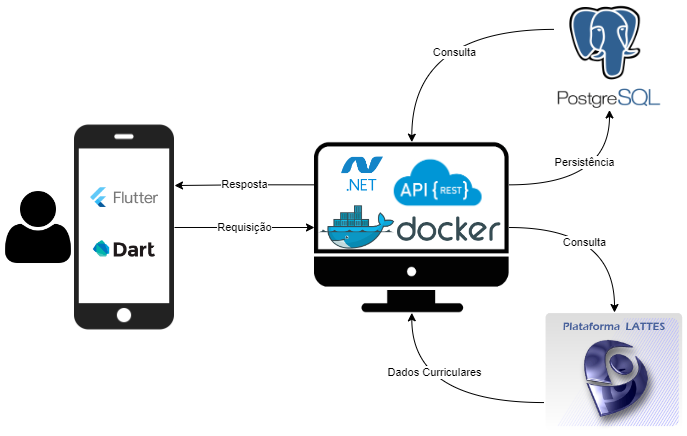
\includegraphics[width=0.8\textwidth]{DiagramaPlataforma}
    \fonte{Autoria Própria}
    \label{fig:diagrama}
\end{figure}